
\section{Introduction}
\label{sec:Introduction}
\textbf{why network virtualization is significant.} Network virtualization is a promising technology to reduce the operating costs and management complexity of networks, and it is receiving an increasing amount of research interest\cite{chowdhury2009network}, as an effective means to share substrate network (SN) infrastructure among several virtual network (VN) service providers so as to improve the utilization of the substrate resources \cite{armbrust2009above,yu2008rethinking}. In the network virtualization environment, provisioning a VN is a promising way to support distributed applications and services which require the coordination of multiple geographically distributed facilities (e.g. storage arrays or computer clusters). With the maturity of the optical network technology and their high-bandwidth and low-latency characteristics, we will be able to deploy a federated computing and networking system (FCNS) \cite{zhang2013effective,papagianni2013optimal}, which interconnects a large number of substrate nodes with optical network managed or controlled integratedly, to enable such large scale distributed applications.

\textbf{what is VN }In network virtualization, the primary entity is the Virtual Network (VN). A VN is a combination of active and passive network elements (network nodes and network links) on top of a Substrate Network (SN). Virtual nodes are interconnected through virtual links, forming a virtual topology.VN also has certain resource requirement, such as computing resources for virtual nodes, specific service network function for virtual nodes and bandwidth resources for virtual links. Each VN request for network resources demand may arrive and leave online. By virtualizing both node and link resources of a SN, multiple virtual network topologies with widely varying characteristics can be created and co-hosted on the same substrate hardware.
 To establish the VN, one needs to embed virtual nodes onto substrate nodes, and virtual edges onto one or more substrate paths\cite{yu2008rethinking} , as well as allocating sufficient substrate resources which should not violate the computing/ bandwidth capacity limits of substrate node/substrate link.



%\textbf{why node failure happern} With infrastructure rapidly becoming virtualized, shared and dynamically changing, it is essential to have strong reliability support from the substrate infrastructure, since a single substrate server or link failure affects several shared virtualized entities. Providing survivability is often linked with over-provisioning both computational and network capacities, and employing load balancing for additional robustness. Such highly survivable systems are good for applications where large discontinuity may be tolerable, e.g. restart of network flows while rerouting over link or node failures, or partial job restarts at node failures. A higher level of fault tolerance is required at applications where some failures have a substantial impact on the current state of the system. For instance, virtual networks with servers which perform admission control, scheduling, load balancing, bandwidth broking, AAA or other NOC operations that maintain snapshots of the network state, cannot tolerate total failures. In master slave/ worker architectures, e.g. MapReduce, failures at the master nodes waste resources at the slaves/workers, we do not talk about the capacity requirement and geographical location requirement of virtual node, and the bandwidth capacity requirement of virtual link in this paper.


\textbf{where failure situation happen} In the multi-tenant network virtualization environment, one challenging problem raised is how to efficiently embed VN requests with various constraints. This is of utmost importance for increasing the utilization of SN resources and infrastructure VN providers’ revenue \cite{koponen2014network}. Survivable virtual network embedding deals with failures in the substrate network, The considering challenges are substrate link failures or substrate node failures, which have to be backed up before the failure or recovered after failure. Failures can occur at different layers in the network. For example at the substrate layer, a fiber cut may cause a substrate network without connectivity. It is shown that 20\% of all failures in an IP backbone are resulting from maintenance activities\cite{markopoulou2004characterization}. About 53\% of the unplanned link failures are due to router-related \cite{markopoulou2004characterization}. In a substrate network, single and also multiple failures can occur, the single failure case happens more often than multiple simultaneous failures. The study \cite{markopoulou2004characterization} states that about 70\% of the unplanned link failures are single link failures. A study \cite{gill2011understanding} about network-related failures in data centers found out that link failures happen about ten times more than node failures per day. Usually node failures are due to maintenance \cite{gill2011understanding}.


\textbf{why Survivability is important. }Survivability is bound to become a more prominent issue as infrastructure providers move toward virtualizing their networks over cheaper commodity hardware \cite{bhatia2008trellis}. Given a failure-prone Internet due to various disruption causes such as maintenance, fiber cut, policy change and misconfiguration, the substrate nodes/links may not operate properly all the time. In case of a substrate node/link failure, all the virtual networks using that node/link will be affected. Therefore, we are concerned with critical virtual nodes and embedding them as an entire infrastructure with survivability guarantees. Survivability is provided in data centers \cite{guo2009bcube} through excessive redundant nodes and links organized in a special way. These works provide survivability but do not customize survivability guarantees to embedded VN.

\textbf{why survivable embedded VN is paramount} However, with network virtualization gaining momentum, the survivability challenges in VNE should also be well investigated\cite{herker2013survey}. In a large networked computing system, hardware and software failures of substrate nodes and communication resources (e.g., links and switching nodes) are norm instead of exception, such as power outages caused by virus attack, disk failures, misconfiguration or fiber cut \cite{xu2012survivable,rahman2010survivable,rahman2013svne,guo2011shared,chen2010resilient}. Such failures will force the virtual node (links) assigned to the substrate node to be migrated/re-embeded to another substrate node at a geographically different location (link disjoint substrate path). This means that, in order to survive from the disruptions due to such failures, one must reserve redundant substrate nodes and bandwidth on fiber links such that after any failure when virtual network request had been embedded in substrate network, there are adequate remaining computing and networking resources to migrate/remap the embedded VN request. In most case, failure occur when VN had been embedded into SN. Accordingly, the problem of minimizing the resources, including computing and communication resources, reserved for VN request to tolerate substrate failures, (hereafter called Survivable embedded VN problem, SeVN) is both critical and challenging. Actually, SeVN problem is quite different with the protection approach
in IP over WDM network by investigating substrate node failure caused virtual node failure problem and employing node migration induced VN remapping as an unique recovery strategy.


\textbf{why happen Survivable embeded Virtual Network Request} The software-defined NFV architecture further offers agile traffic steering and joint optimization of network functions and resources.
%When a survivable request of virtual network is coming, survivable virtual network requests are associated with node's service functions.
In any real virtual networks, any nodes of virtual network  are deployed with a service function and the substrate node support a service functions set for virtual node implementing. After virtual network is embedded into substrate network, a working node of substrate network fail so that  multiple virtual node do not work, therefore we should obtain survivable eVN to be embedded into substrate network so that recovery from the failure even though one or multiple nodes of virtual network failed because these virtual node corresponding substrate node fail. The augmented(alternated) nodes of survivable embedded virtual network are embedded into substrate network ultimately.
%the augmented nodes have specific service functions similarly as shown in Fig.\ref{fig:VNmapSN}.

\begin{figure*}
  \centering
  % Requires \usepackage{graphicx}
  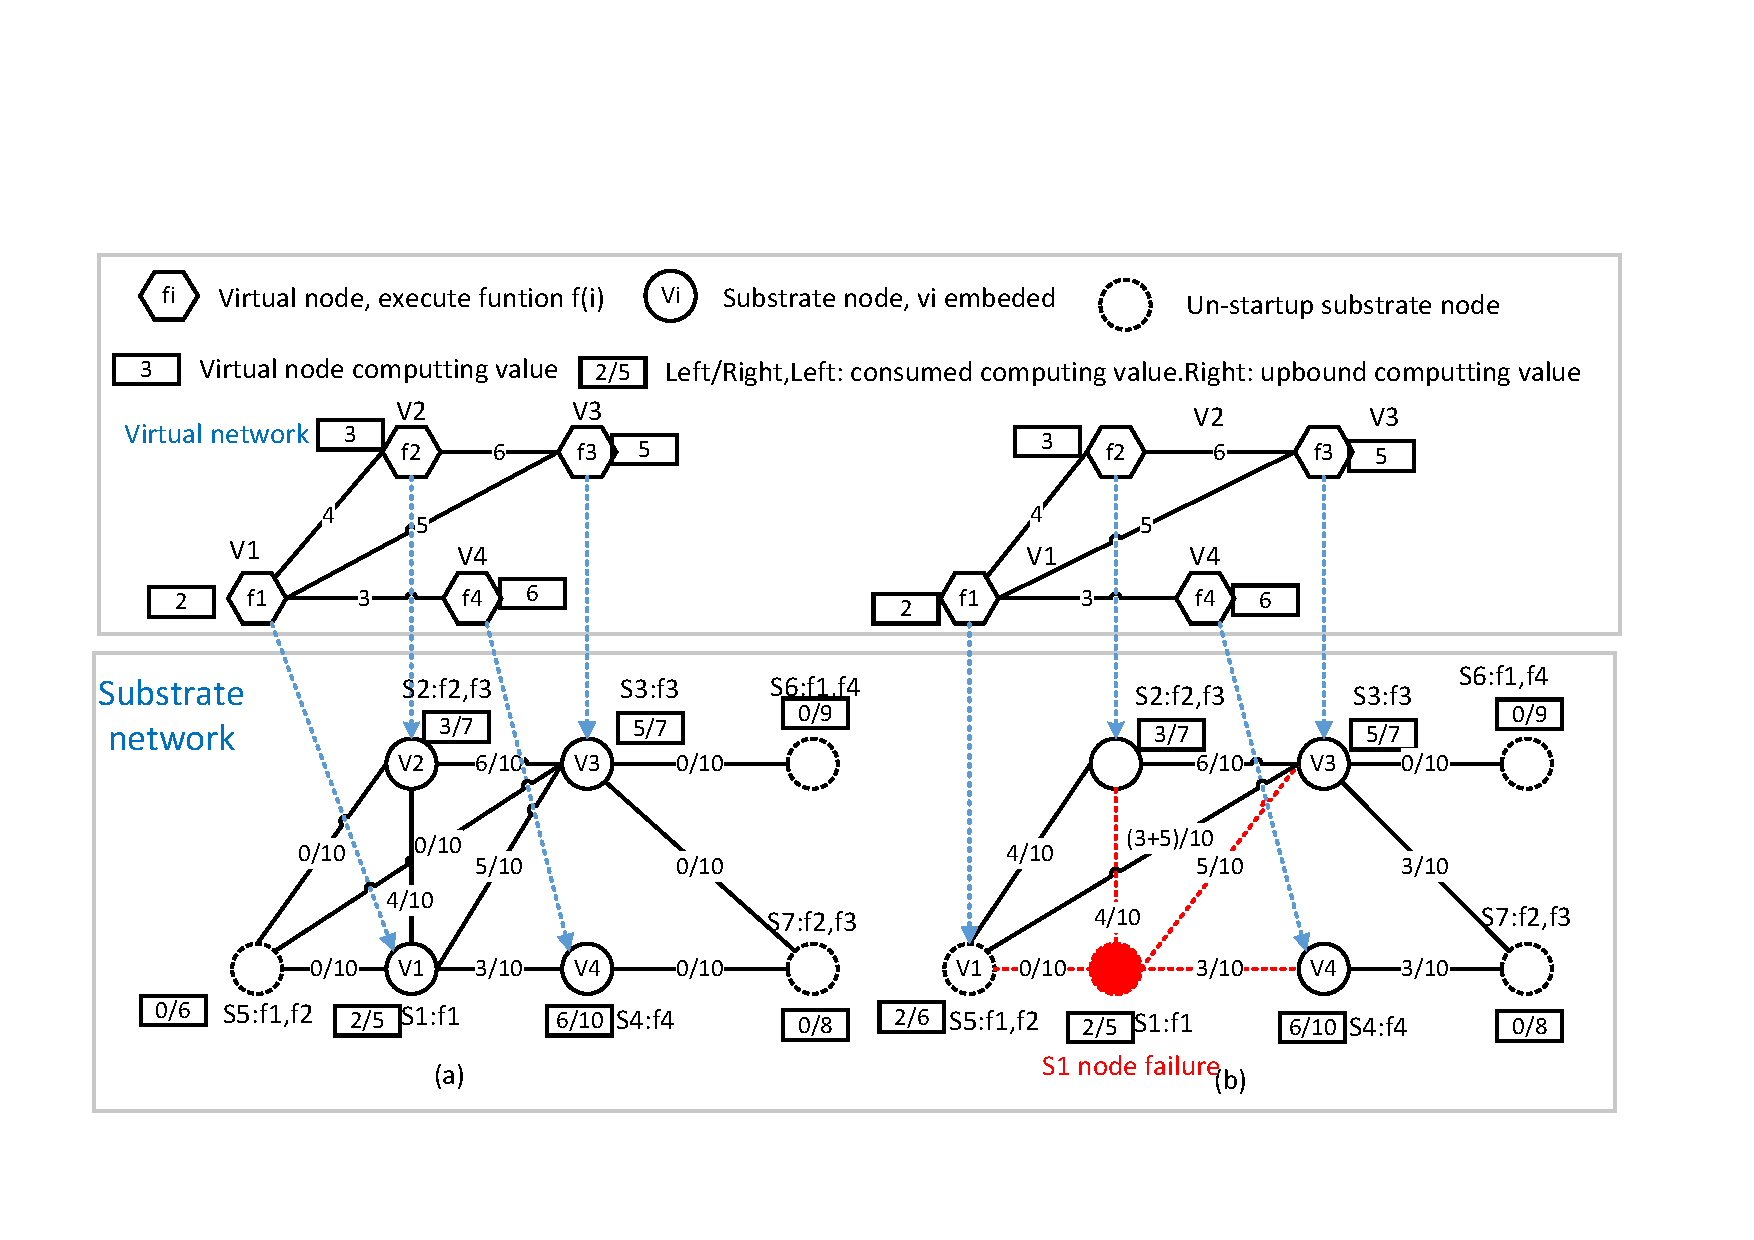
\includegraphics[width=5in]{Fig/VNmapSN}\\
  \caption{function virtual network (VN) embedding and one node failure}\label{fig:VNmapSN}
\end{figure*}



There are two main survivability methods: \textbf{proactive protection} and \textbf{reactive restoration} \cite{ramamurthy2003survivable}. Failure protection is done in a proactive way to reserve the backup resources before any failure happens. Reactive mechanisms, which are called restoration mechanisms, react after the failure occurs and start the backup restoring mechanism. However, some data loss is possible in the reactive case. To survive a substrate link failure, precomputed alternative paths in VN are used in general and the bandwidths are allocated before or after a failure. For instance, the reactive detour solution was employed after a substrate link failure in \cite{rahman2010survivable}, while authors\cite{rahman2013svne,guo2011shared} proposed a proactive backup approach (considering the backup resources sharing) to avoid service disruption in reactive restoration approach and improve the substrate resource utilization.

In the other hand, There exist two kinds of backups for the protection scheme: \textbf{dedicated backup} or \textbf{shared backup}. In shared backup, the resources for the backup may be shared with other backups. In the dedicated case the backup resources are not shared for other backups.


In terms of SeVN capable of recovering/re-embedding the virtual nodes after a substrate node failure, there are two basic approaches: \textbf{Failure Dependent Protection} (FDP \cite{yu2010survivable} and \textbf{Failure Independent Protection} (FIP \cite{yeow2011designing}) , and the differences between them are as follows. In FIP, a host (substrate) node is assigned and dedicated to backup all working host (substrate) nodes. That is, no matter which working host node fails, the affected virtual node will be migrated to the only one backup host node. On the other hand, with FDP, each working host node can have a different backup host node under different failure scenarios. In fact, after a failure, even an unaffected virtual node may be migrated from a working host node to its corresponding backup host node, as a result of re-embedding the entire virtual graph. In other words, FDP could provide more flexibility in survivable VN designing by allowing virtual nodes migrating freely when processing a substrate node failure, so FIP could be considered as a special case of FDP and FDP is expected to use fewer resources at the cost of more virtual nodes migrations when processing a substrate node failure.


Guarantying integration of topological structure of virtual network request is more important than node migration cost when substrate node failure. As nodes often represent expensive components (servers) and edges represent less expensive interconnections (links) \cite{armbrust2009above,yu2010survivable}, most attention has been devoted to node faults, i.e., the removal of nodes (and their incident edges), rather than edge faults where only edges are removed. The node failure type we focus in this paper is independent node failures. multiple independent or dependent failure nodes problem could be discussed Sec.\ref{sec:multiplePhysicalNodeFailure}.



Through synchronization \cite{bressoud1996hypervisor,cully2008remus} and migration techniques \cite{clark2005live,wang2008virtual} on virtual machines and routers, we suppose that every virtual network have specific service functions\cite{houidi2009virtual}, which is referred from substrate resource attribute or node/link location-constrain, in addition that fault tolerant can be introduced at the virtualization layer \cite{yeow2011designing,qu2016delay}.



Substrate resources are described in terms of functional and non-functional
attributes:
\begin{itemize}
  \item Functional attributes: define characteristics and properties of the substrate resources ns and ls including static parameters like node type (e.g. router, switch), node processor type and capacity (e.g. CPU, network processor), link/path type (e.g. VLAN, L3/L2 VPN), network interface type and number, geographic location, cost and so on.
  \item Non-functional attributes: specify criteria and constraints related to the substrate resources including dynamic (real-time) parameters like available node capacity (CPU), available link capacity (bandwidth), actual QoS parameters, geographic coordinates, etc.
\end{itemize}





%
%\begin{table}
%\centering
%\begin{tabular}{cc}
%\hline
%Term & Description \\
%$G(V,E,S)$ & $G(V,E,S)$ denotes the Virtual Network, consisting of nodes V, links E and service functions\\
%$B(V,S)$ & $B(V,S)$ denotes the Backup nodes set, consisting of nodes V and service functions S which is corresponding to every nodes \\
%\hline
%\end{tabular}
%\caption{terminology used throughout this paper}\label{tab:term}
%\end{table}

We conduct both theoretical analysis and simulation-based performance evaluation, which have validated the effectiveness of our proposed algorithms. Our main contributions are summarized as follows:
\begin{itemize}
  \item To the best of our knowledge, we are the first to study the survivable network embedding problem with node computation, link bandwidth and node function type constraint. Considering joint node mapping and link mapping optimization.
  \item We propose a graph decomposition heuristic  algorithm that finds the most resource-efficient survivable virtual network embedding for each virtual network request.
  \item We further propose a pseudo-polynomial time dynamic program algorithm that reduces the time complexity of star matching problem, yet optimize the space complexity of the dynamic program method.
  \item We use extensive experiments to evaluate the performance of our proposed algorithms.
\end{itemize}



The organization of this paper is as follow. In the next section, we briefly describe the background, notations and our problem in Sec.\ref{sec:Problem description}. Finally, we evaluate and validate my supposed algorithm through simulation in Sec.\ref{sec:Evaluation}.

